%%%%%%%%%%%%%%%%%%%%%%%%%%%%%%%%%%%%%%%%%%%%%%%%%%%%%%%%%%%%%%%%%%
%%%%%%%% ICML 2015 EXAMPLE LATEX SUBMISSION FILE %%%%%%%%%%%%%%%%%
%%%%%%%%%%%%%%%%%%%%%%%%%%%%%%%%%%%%%%%%%%%%%%%%%%%%%%%%%%%%%%%%%%

% Use the following line _only_ if you're still using LaTeX 2.09.
%\documentstyle[icml2015,epsf,natbib]{article}
% If you rely on Latex2e packages, like most modern people use this:
\documentclass{article}

% use Times
\usepackage{times}
% For figures
\usepackage{graphicx} % more modern
%\usepackage{epsfig} % less modern
\usepackage{subfigure} 

% For citations
\usepackage{natbib}

% For algorithms
\usepackage{amsmath}
%\usepackage{algorithm}
%\usepackage{algorithmic}
\usepackage{bm}

% As of 2011, we use the hyperref package to produce hyperlinks in the
% resulting PDF.  If this breaks your system, please commend out the
% following usepackage line and replace \usepackage{icml2015} with
% \usepackage[nohyperref]{icml2015} above.
\usepackage{hyperref}

% Packages hyperref and algorithmic misbehave sometimes.  We can fix
% this with the following command.
\newcommand{\theHalgorithm}{\arabic{algorithm}}

% Employ the following version of the ``usepackage'' statement for
% submitting the draft version of the paper for review.  This will set
% the note in the first column to ``Under review.  Do not distribute.''
\usepackage[accepted]{icml2015} 

% Employ this version of the ``usepackage'' statement after the paper has
% been accepted, when creating the final version.  This will set the
% note in the first column to ``Proceedings of the...''
%\usepackage[accepted]{icml2015}


% The \icmltitle you define below is probably too long as a header.
% Therefore, a short form for the running title is supplied here:
\icmltitlerunning{Under review as a conference paper for ICML 2016 workshop on Human Interpretability in Machine Learning}

\begin{document} 

\twocolumn[
\icmltitle{Not Just A Black Box: \\ 
           Interpretable Deep Learning by Propagating Activation Differences}

% It is OKAY to include author information, even for blind
% submissions: the style file will automatically remove it for you
% unless you've provided the [accepted] option to the icml2015
% package.
\begin{center}{ {\bf Avanti Shrikumar$^1$} (avanti@stanford.edu), {\bf Peyton Greenside$^2$} (pgreens@stanford.edu)\\{\bf Anna Shcherbina$^2$} (annashch@stanford.edu), {\bf Anshul Kundaje$^{1,3}$} (akundaje@stanford.edu)}\end{center}
\icmladdress{1. Department of Computer Science, Stanford University, CA, USA\\2. Biomedical Informatics, Stanford University, CA, USA\\3. Department of Genetics, Stanford University, CA, USA}

% You may provide any keywords that you 
% find helpful for describing your paper; these are used to populate 
% the "keywords" metadata in the PDF but will not be shown in the document
\icmlkeywords{DeepPAD, deep learning, interpretability, interpretable, neural networks, importance, feature importance, ICML}

\vskip 0.3in
]

\begin{abstract} 
A common criticism of neural networks is their lack of interpretability or ``black box" nature. This is a major barrier to adoption in application domains such as biology, where interpretability is important. Here we present DeepPAD (Propagating Activation Differences), an intuitive and effective method for scoring the contributions of inputs to the output of a neural network. DeepPAD compares the activation of each neuron to its `reference activation', and assigns a contribution score to each of the neuron's inputs proportionally to how the inputs differ from their own `reference activations'. We apply DeepPAD to models trained on natural images as well as models trained on genomic sequences. We show that DeepPAD correctly identifies important features in both cases and has significant advantages over gradient-based methods.
\end{abstract} 

\section{Introduction}
\label{introduction}

As neural networks become increasingly popular, their reputation as a ``black box" presents a barrier to adoption in fields where interpretability is paramount. Understanding the features that lead to a particular output builds trust with users and can lead to novel scientific discoveries. A common approach is to leverage the gradients of a particular output with respect to the individual inputs (Simonyan et al. - cite) - however, such approaches are limited because activation functions such as Rectified Linear Units (ReLUs) have a gradient of zero when they are not firing, yet a ReLU that does not fire can still carry information - particularly if the associated bias is positive (which means that in the absence of any input, the ReLU does fire). Similarly, sigmoid or tanh activations are popular choices for the activation functions of gates in memory units of recurrent neural networks such as GRUs and LSTMs (cite), but these activations have a near-zero gradient at high or low inputs even though such inputs can be very significant.

In this paper, we present a general method for assigning feature importance that focuses on the difference between a neuron's activation and its `reference' activation, where the reference activation is the activation that the neuron has when the network is provided a `reference input'. The reference input is defined on a domain-specific basis according to what is appropriate for the task at hand. This circumvents the aforementioned limitation of gradient-based approaches because, rather than relying on the local gradient at the point of activation, the activation is simply compared to its reference value. In the case of a ReLU that fires when provided the reference input (as is typically the case for ReLUs that have a positive bias), our method assigns a negative `difference from reference' when the ReLU does not fire. Similarly, in the case of a sigmoidal unit which has an output of $0.5$ when provided the reference input, our method would assign a positive `difference from reference' when the sigmoidal unit has an output near $1$, even though the gradient at that output is negligible.

\section{DeepPAD Method}
\label{PAD}

We denote the contribution of $x$ to $y$ as $C_{xy}$. Let the activation of a neuron $n$ be denoted as $A_n$. Further, let the \emph{reference} activation of neuron $n$ be denoted $A_n^0$, and let the $A_n - A_n^0$ be denoted as $\delta_n$. We define our contributions $C_{xy}$ to satisfy the following properties.

\subsection{Summation to $\delta$}

For any set of neurons $S$ whose activations are minimally sufficient to compute the activation of $y$ (that is, if we know the activations of $S$, we can compute the activation of $y$, and there is no set $S' \subset S$ such that $S'$ is sufficient to compute the activation of $y$ - in layman's terms, $S$ is a full set of non-redundant inputs to $y$), the following property holds:
\begin{equation}
\sum_{s \in S} C_{sy} = \delta_y
\end{equation}
That is, the sum over all the contributions of neurons in $S$ to $y$ equals the difference-from-reference of $y$.

\subsection{Linear composition}

Let $O_x$ represent the output neurons of $x$. The following property holds:\\
\begin{equation}
C_{xy} = \sum_{o \in O_x} \frac{C_{xo}}{\delta_o}C_{oy}
\end{equation}
In layman's terms, each neuron `inherits' a contribution through its outputs in proportion to how much that neuron contributes to the difference-from-reference of the output.

\subsection{Backpropagation Rules}

We show that the contributions as defined above can be computed using the following rules (which can be implemented to run on a GPU). The computation is reminiscent of the chain rule used during gradient backpropagation, as equation $2$ makes it possible to start with contribution scores of later layers and use them to find the contribution scores of preceding layers. To avoid issues of numerical stability when $\delta_n$ for a particular neuron is small, rather than computing the contribution scores explicitly, we instead compute \emph{multipliers} $m_{xy}$ that, when multiplied with the difference-from-reference, give the contribution:
\begin{equation}
m_{xy} \delta_x = C_{xy}
\end{equation} 
Let $t$ represent the target neuron that we intend to compute contributions to, and let $O_x$ represent the set of outputs of $x$. We show that:
\begin{equation}
m_{xt} = \sum_{y \in O_x} m_{xy}m_{yt}
\end{equation} 
The equation above follows from the linear composition property and the definition of the multipliers, as proved below:
\begin{equation}
\begin{aligned}
C_{xt} &= \sum_{y \in O_x} \frac{C_{xy}}{\delta_y}C_{yt}\\
m_{xt} \delta_x &= \sum_{y \in O_x} \frac{C_{xy}}{\delta_y}(m_{yt} \delta_y)\\
                         &= \sum_{y \in O_x} C_{xy}m_{yt}\\
m_{xt} &= \sum_{y \in O_x} \frac{C_{xy}}{\delta_x}m_{yt}\\
m_{xt} &= \sum_{y \in O_x} m_{xy} m_{yt}
\end{aligned}
\end{equation} 

In the equations below, $I_y$ denotes the set of inputs of $y$.

\subsubsection{Affine functions}
Let
\begin{equation}
A_y = \left(\sum_{x \in I_y} w_{xy} A_x\right) + b  
\end{equation}
Then
\begin{equation}
\begin{aligned}
m_{xy} &= w_{xy}
\end{aligned}
\end{equation}

{\bf Proof.} We show that
\begin{equation}
\delta_y = \sum_{x \in I_y} m_{xy} \delta_x 
\end{equation}
Using the fact that $A_n = A_n^0 + \delta_n$, we have:
\begin{equation}
\begin{aligned}
(A_y^0 + \delta_y) &= \left(\sum_{x \in I_y} w_{xy} (A_x^0 + \delta_x) \right) + b \\
                              &= \left(\sum_{x \in I_y} w_{xy} A_x^0 \right) + b + \sum_{x \in I_y} w_{xy} \delta_x
\end{aligned}
\end{equation} 
We also note that the reference activation $A_y^0$ can be found as follows:
\begin{equation}
A_y^0 = \left(\sum_{x \in I_y} w_{xy} A_x^0 \right) + b
\end{equation}
Thus, canceling out $A_y^0$ yields:
\begin{equation}
\begin{aligned}
\delta_y &= \sum_{x \in I_y} w_{xy} \delta_x\\
             &= \sum_{x \in I_y} m_{xy} \delta_x
\end{aligned}
\end{equation} 

\subsubsection{Max pooling over convolutional filters}

We consider the case of maxpooling over a set of neurons in a convolutional layer which all belong to the same convolutional filter:
\begin{equation}
A_y = \max_{x \in I_y} A_x
\end{equation}
We make the assumption that all instances of a single convolutional filter have the same reference activation, i.e. $A_x^0$ is the same for all $x$ in $I_y$ (this would not hold if the chosen reference input were not uniform across all positions; the appropriate multiplier in that situation can be computed easily, but is omitted here for brevity). Then we have:
\begin{equation}
m_{xy} = \bm{1}\{A_x = A_y\}
\end{equation}
Where $\bm{1}\{\}$ is the indicator function. If a symbolic computation package is used, then the gradient of $y$ with respect to $x$ can be used in place of $\bm{1}\{A_x = A_y\}$.

{\bf Proof.} Because $A_x^0$ is assumed to be the same for all $x$, we have that $A_y^0 = A_x^0$. As $A_y = A_y^0 + \delta_y$, we get:
\begin{equation}
\begin{aligned}
\delta_y &= A_y - A_y^0\\
             &= A_y - A_x^0\\
             &= \bm{1}\{A_x = A_y\} (A_x - A_x^0)\\
             &= \bm{1}\{A_x = A_y\} \delta_x\\
             &= m_{xy} \delta_x
\end{aligned}
\end{equation}

\subsubsection{Individual nonlinearity}

Here we describe the rule for nonlinear transformations such as the ReLU, sigmoid and tanh which are applied to individual inputs, typically following some affine transformation. We have:
\begin{equation}
A_y = f(A_x)
\end{equation}
Where $f$ is the nonlinear transformation. When $\delta_x$ is large in magnitude, we can compute $m_{xy}$ according to its definition as follows:
\begin{equation}
m_{xy} = \frac{\delta_y}{\delta_x}
\end{equation}
When $\delta_x$ is small, the term on the right approaches $\frac{0}{0}$. However, as $\delta_y \rightarrow 0$ as $\delta_x \rightarrow 0$, we have:
\begin{equation}
\lim_{\delta_x \rightarrow 0} \frac{\delta_y}{\delta_x} = \frac{d \delta_y}{d \delta_x}
\end{equation}
Thus, when $\delta_x$ is close to zero, $m_{xy}$ is simply the derivative of $\delta_y$ with respect to $\delta_x$. Because $\delta_n = A_n - A_n^0$ and $A_n^0$ is a constant, this is the same as $\frac{dA_y}{dA_x}$ when $\delta_x$ is near $0$.

\subsubsection{Softmax activation}

Let ${t_1, t_2...t_n}$ represent the output of a softmax transformation on the nodes ${y_1, y_2...y_n}$, such that:
\begin{equation}
A_{t_i} = \frac{e^{A_{y_i}}}{\sum_{i' = 1}^n e^{A_{y_i'}}} 
\end{equation}
Here, $A_{y_1}...A_{y_n}$ are affine functions of their inputs. Let $x$ represent a neuron that is an input to $A_{y_1}...A_{y_n}$, and let $w_{xy_i}$ represent the coefficient of $A_x$ in $A_{y_i}$. Because $A_{y_1}...A_{y_n}$ are followed by a softmax transformation, if $w_{xy_i}$ is the same for all $y_i$ (that is, $x$ contributes equally to all $y_i$), then $x$ effectively has zero contribution to $A_{t_i}$. This can be observed by substituting $A_{y_i} = w_{xy_i}A_x + r_{y_i}$ in the expression for $A_{t_i}$ and canceling out $e^{w_{xy_i}A_x}$ (here, $r_{y_i}$ is the sum of all the remaining terms in the affine expression for $A_{y_i}$)
\begin{equation}
\begin{aligned}
A_{t_i} &= \frac{e^{A_{y_i}}}{\sum_{i' = 1}^n e^{A_{y_i'}}}\\
           &= \frac{e^{w_{xy_i}A_x + r_{y_i}}}{\sum_{i' = 1}^n e^{w_{xy_i'}A_x + r_{y_i'}}}\\
           &= \frac{e^{w_{xy_i}A_x + r_{y_i}}}{\sum_{i' = 1}^n e^{w_{xy_i}A_x + r_{y_i'}}}\\
           &= \frac{e^{r_{y_i}}}{\sum_{i' = 1}^n e^{r_{y_i'}}} 
\end{aligned}
\end{equation}
One way to ensure that $C_{xt}$ is zero if $w_{xy_i}$ is the same for all $y_i$ is to set:
%\begin{equation}
%\begin{cases}
%C_{y_i' t_i} &= \frac{n-1}{n} \delta_t_i' & \text{for} i' = i
%\end{cases}
%\end{equation}

\subsection{A note on final activation layers}

\subsection{A note on weight normalization for constrained inputs}

\section{Results}

We apply DeepPAD to models that classify genomic sequences. The positive class requires that two particular DNA patterns - 'GATA' and 'CAGATG' - appear in the sequence together. They may appear at any spacing. The negative class has just one of the two patterns appearing either once or twice, also at any spacing. We simulate 20,000 sequences of length 200 for the positive set and 40,000 sequences for the negative set split equally between the two patterns. Outside the core patterns we randomly sample the remaining sequence with equal frequency for the four bases A, C, G and T. We trained a model on these sequences with 20 convolutional filters of length 15 with a PReLU and a max pool layer of stride 50 followed by two fully connected layers of size 200. This model performs well with auROC of 0.907. The misclassified examples primarily occur when one of the patterns erroneously arises in the randomly sampled background.  % We use dropout with probability 0.3, l1 activity regularization (1e-7) and a weight norm of 7 on the fully connected layers. 

We then run DeepPAD to assign an importance score to each base in the correctly predicted sequences. We also use a gradient-based method for comparison. In Figure 1 we illustrate that DeepPAD clearly discovers both patterns and assigns them large importance scores as compared to the surrounding sequence. The gradient-based method discovers only one of the two important patterns despite a correct prediction.

\begin{figure}[!htmb]
\begin{center}
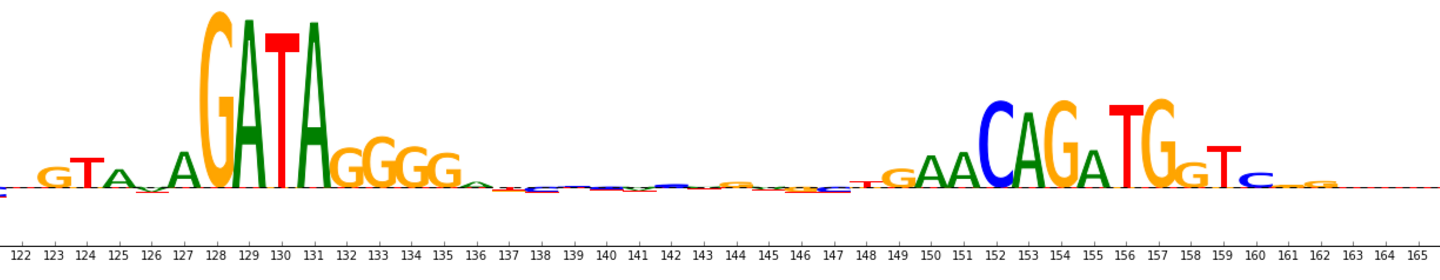
\includegraphics[scale=0.3]{DeepPADSequence2.png}
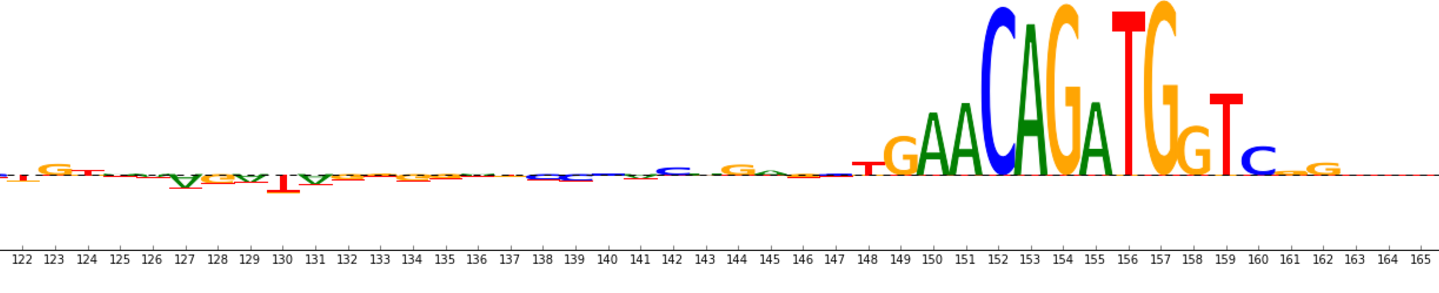
\includegraphics[scale=0.3]{GradientSequence2.png}
\caption{DeepPAD scores (top) and gradient-based scores (bottom) are plotted for each position in the DNA sequence and colored by the DNA base.}
\end{center}
\end{figure}
 

\section{Discussion}

\section{References}

\end{document} 

% This document was modified from the file originally made available by
% Pat Langley and Andrea Danyluk for ICML-2K. This version was
% created by Lise Getoor and Tobias Scheffer, it was slightly modified  
% from the 2010 version by Thorsten Joachims & Johannes Fuernkranz, 
% slightly modified from the 2009 version by Kiri Wagstaff and 
% Sam Roweis's 2008 version, which is slightly modified from 
% Prasad Tadepalli's 2007 version which is a lightly 
% changed version of the previous year's version by Andrew Moore, 
% which was in turn edited from those of Kristian Kersting and 
% Codrina Lauth. Alex Smola contributed to the algorithmic style files.  


